\documentclass[a4paper, 11pt]{article}

\usepackage[utf8]{inputenc}
%\usepackage[french]{babel}
\usepackage[T1]{fontenc}
\usepackage{amssymb}
\usepackage{amsmath}
\usepackage{mathpartir}
\usepackage{mathtools}
\usepackage{caption}
\usepackage{amsthm}
\usepackage{stmaryrd}
\usepackage{titlesec}
\usepackage{algorithm}
\usepackage{algpseudocode}
\usepackage{framed}
\usepackage{forest}
\usepackage{tikz}
\usetikzlibrary{calc,
                positioning}

\topmargin= .5cm
\textheight= 20cm
\textwidth= 32cc
\baselineskip=16pt

\evensidemargin= .9cm
\oddsidemargin= .9cm

\newtheorem{theorem}{Theorem}
\newtheorem{lemma}[theorem]{Lemma}
\newtheorem{corollary}[theorem]{Corollary}
\newtheorem{definition}[theorem]{Definition}
\newtheorem{example}[theorem]{Example}
\newtheorem*{notation}{Notation}
\newtheorem*{remark}{Remark}

\newcommand{\ie}{ \textit{i.e.} }

\DeclareMathOperator{\nf}{NF}

\title{Master Internship's report}
\author{Vladislas de Haldat\\\small{Supervised by Simon Guilloud and Viktor Kunčak, EPFL}}

\begin{document}

    \maketitle

	\subsection*{General context}
	With the advent of computers in the second half of the XXth century, the question whether 
	machines are able or not to \textit{reason} and to automatically prove mathematical statements 
	rised from its ashes. In the 60s, a convenient method has been exhibited by Davis and Putnam
	and has proved itself in term of efficiency so far. It consists in transforming the problem one
	wants to solve into a conjunctive normal form. This normal form allows the computer to
	efficiently derive a proof using a couple of logical rules only. Doing that, we are in fact
	reducing the problem to the SAT problem that is known to be NP complete. This implies that,
	supposing $P\neq NP$, no deterministic algorithm is able to decide the problem in polynomial
	time. However, the use of heuristics, that is to say, the use of non-deterministic algorithms
	helps to improve time spent to solve a SAT problem. The conjunctive normal form is, of course,
	not the only normal form that has been tried to get better performance to automatic reasonning.
	In the beginning of the 2000s, researchers tried to take advantage of the negation normal form.
	The singularity of this normal form is that the negation operator is only applied on litterals.
	According to rewriting rules of boolean algebra, one can derive the negative normal form of a
	given formula in linear time. However, those proposed algorithms never reached performances
	comparable to the former algorithms, based on the conjunctive normal form. The following report
	is about a way to improve the current state of the art of modern SAT solvers in two different
	ways. On one hand, we look to improve the preprocessing of formulas by applying a new normal
	form that gets rid of some redundancy, making the formulas smaller. On the other hand, we explore
	a new set of rules that helps to improve solving performances on some kind of hard problems.

	%What is the report about ? Where does the problem come from ? What is the state of the art in that area ?

	\subsection*{Research problem}
	In the following, we tackle a generalization of classical logic that is called 
	\textit{orthologic} (OL for short) and we try to take advantage of
	some of its properties to derive an efficient solving algorithm on some specific class of 
	problems. Indeed, the SAT solvers are good in average, but they can be very slow on classes of
	problems that are intuitively easy or that have enough structure to be efficiently decided by an
	algorithm. We improve the state of the art solvers by using alternatie technique to solve these
	specific classes. 
%	The main motivation behind that research is the improvement of performance of
%	automatic reasonning tools and, in particular, of SAT solvers. The goal is to integrate our
%	resulting algorithm in the core of a SAT solver to improve its efficiency on certain class of
%	problems. Although the problem of improving current SAT solvers is not new, we address it in a
%	completely different way by looking deeper in the logical structure to extract interesting
%	properties to our purposes.

	%What specific question(s) have you studied ?
	%What motivates the question? What are its applications/consequences?
	%Is it a new problem ?
	%Why did you choose this problem?
	%If so, why are you the first researcher in the universe to consider it?
	%If not, why did you think that you could bring an original contribution?

	\subsection*{Your contribution}
	The contributions of this report are two fold. First, we show that the use of another normal
	form, before transforming a formula into CNF, can improve the solving performances of SAT 
	solvers.
	Second, and this is the main contribution, we propose an efficient proof-search algorithm based 
	on a proof system of the generalization of classical logic we use. We showed that it is correct 
	and that it admits a cubical worst-case complexity. To evaluate the performances, we studied the 
	specific class of problems of circuit
	equivalence modulo renaming. This happens to be a class of problems SAT solvers struggle to 
	deal with.
	However, we showed that we can easely encode it into the framework of our proof system and 
	thus, ask a proof for it in our proof system.

	%What is your answer to the research problem?

	%Please remain at a high level; technical details should be given in the main body of the report.
	%Pay special attention to the description  of the \emph{scientific} approach.

	\subsection*{Arguments supporting its validity}
	The results we have gathered come with benchmarks evaluation on different kind of problems.
	Concerning the proof-search algorithm we exhibited, we provide, in addition to the benchmarking, 
	proofs of its correctness and of its worst case complexity. Furthermore, let us note that our
	results do not rely on any kind of assumptions but rather on work of previous peers on the topic.

	%What is the evidence that your solution is a good solution?
	%(Experiments? Proofs?)

	%Comment on the robustness of your solution: does it rely on assumptions, and if so, to what extent?

	\subsection*{Summary and future work}
	To sum up, we propose two ways to improve the current state of the art of SAT solvers. 
	On way handles the preprocessing of the formulas while the other handles the proof-search
	algorithm for certain class of problems. Next, the immediate step to do is
	to implement our algorithm within an existing simple SAT solver, such as Minisat, and test
	whether the performances are improved, compared to the original version. There are many questions
	that stand further. The main one is to study the lifting to first order logic and the way to 
	adapt our results to specific theories such as bit vectors, lists, arrays etc.

	%What did you contribute to the area?
	%What comes next?
	%What is a good \emph{next} step or question?

	\subsection*{Acknowledgements}
	Before anything else, I'd like to warmly thank Simon and Viktor for having had me in their 
	laboratory at EPFL and, moreover, for the support they provided me to study that concealed, yet
	rich topic of orthologic. Many thanks also to Auguste, Samuel and Sankalp for the help and 
	the nice discussions we had.

	\newpage
    \section{Introduction}
    In this section, we shall introduce the key concepts and the notations that will be mainly used in
    the present report. Few years after the advent of quantum mechanics, a rigorous mathematical 
    foundation has been proposed by von Neumann~\cite{30573279-e8ec-3f1e-b0ba-eaf73275f821} leading, 
    after some observations~\cite{2c73be7a-3de4-3824-8e11-49ebe4b183e4}, to a 
    non-classical logical structure that would get rid of the distributivity identities. 
    The associated algebra to such a structure is the class of the so
    called \textit{orthomodular lattices}, rather than the classical boolean algebras. This gave birth 
    to a new
    field of logic called the \textit{quantum logic}. The term of \textit{orthologic} has first been 
    introduced
    by Goldblatt~\cite{865e9aad-6de2-3b16-9861-412a9b18e683} to refer to the logic that corresponds to
    the algebraic class of \textit{orthocomplemented lattices} or \textit{ortholattices} for short.
    Those are a generalization of the boolean algebras and, in particular, give up the axiom of 
    distributivity. For ortholattices are weaker than orthomodular lattices, it is also
    often called the \textit{minimal quantum logic}. 
    First, we shall give some basic notions about lattices, after what, we will introduce the underlying 
    notion of ortholattices. Then we will take a closer look to
    a normal form of the orthologic and, finally, we will present a proof system for orthologic.
    \begin{definition}[Lattice]
	    A lattice $\langle L,\wedge,\vee\rangle$ is an algebraic structure where $L$ is a set and 
	    $\wedge$ and $\vee$ are two binary, commutative, associative and idempotent operations 
	    satisfying the
	    following axiomatic identities, also called \textit{absorption laws}.
	    \begin{align*}
		    a\vee(a\wedge b)&=a\\
		    a\wedge(a\vee b)&=a
	    \end{align*}
	    Moreover, the lattice is said to be bounded when there exists two elements $\bot$ and $\top$
	    such that $x\vee\top=\top$, $x\wedge\bot=\bot$ and $x\vee\bot=x\wedge\top=x$.
    \end{definition}
    \begin{remark}
    A lattice can also be seen as a partial order, in which case, we associate it the following order
    relation.
    \[
	a\leq b\Leftrightarrow a=(a\wedge b)
    \]
    Or, equivalently, if and only if $b=(a\vee b)$.	
    \end{remark}
    \begin{definition}[Generated lattice]
	    A lattice is said to be generated by a family of elements $(X_i)$ if its elements consist in
	    the $X_i$'s and their finite combinations by $\wedge$ and $\vee$.
    \end{definition}
    \begin{definition}[Free lattice]
	    A free lattice generated by a family of elements $(X_i)$ is a lattice in which there is no
	    other laws of equality than the ones derived by the axiomatic identities of the lattice.
    \end{definition}
    \subsection{Ortholattices}
    As for classical logic with boolean algebras or, similarly, intuitionnistic logic with Heyting 
    algebras, orthologic also has an underlying algebraic structure that we call 
    \textit{orthocomplemented lattices} or \textit{ortholattices} for short. To introduce it, we need
    a very last notion that is the \textit{orthocomplement}.
    \begin{definition}[Orthocomplement]
	    An orthogonal complementation (or orthocomplement for short) on a bounded lattice $L$ is a
	    function $\neg:L\rightarrow L$ that respects the complement law $\neg a\vee a=\top$ and
	    $\neg a\wedge a=\bot$, the involution law $\neg\neg a=a$ and, finally, the order-reversing
	    law $a\leq b$ implies $\neg b\leq\neg a$.
    \end{definition}
    We now have all the ingredients to properly define the ortholattices. An \textit{ortholattice} is a 
    bounded
    lattice that comes with an \textit{orthocomplement} $\neg$. We show, in the table~\ref{tab_ax},
    an axiomatization of ortholattices that is a sum up of all the axiomatic identities we have seen so
    far. With that set, one can show that boolean algebras are special cases of ortholattices, in 
    particular, the cases where distributivity holds.
    \begin{table}[h]
	    \caption{Axiomatization of ortholattices}
	    \label{tab_ax}
    \begin{center} 
	    \begin{tabular}{ c|c }
		    $x\vee y=y\vee x$&$x\wedge y=y\wedge x$\\
		    $x\vee(y\vee z)=(x\vee y)\vee z$&$x\wedge(y\wedge z)=(x\wedge y)\wedge z$\\
		    $x\vee x=x$&$x\wedge x=x$\\
		    $x\vee\top=\top$&$x\wedge\bot=\bot$\\
		    $x\vee\bot=x$&$x\wedge\top=x$\\
		    $\neg\neg x=x$& \\
		    $x\vee\neg x=\top$&$x\wedge\neg x=\bot$\\
		    $\neg(x\vee y)=\neg x\wedge\neg y$&$\neg(x\wedge y)=\neg x\vee\neg y$\\
		    $x\vee(x\wedge y)=x$&$x\wedge(x\vee y)=x$
	    \end{tabular}
    \end{center}
    \end{table}
    \\
    Furthermore, note that this set of axiom is not minimal, but it highlights the duality between 
    $\wedge$ and
    $\vee$, as well as the duality between $\bot$ and $\top$. For the minimal set of axioms of 
    ortholattices, refer to~\cite{MCCUNE1998285}. We shall write $a=b$ if and only if $a\leq b$ 
    and $b\leq a$. Remark also that ortholattices are weaker than orthomodular lattices since they do 
    not admit the following law as an axiom:
    \[
	    a\leq b\Rightarrow a\vee(\neg a\wedge b)=b
    \]
    In the following of the report, we will denote orthologic by the acronym OL. Let us illustrate
    ortholattices through the following example. 
    \begin{example}
	    \label{example1}
	    The following is an ortholattice, while it is not a boolean algebra.
	    \begin{center}
	    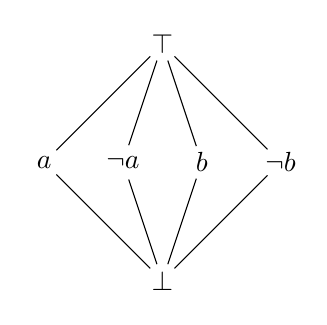
\begin{tikzpicture}[
node distance = 15mm and 10mm, on grid,
every node/.style = {circle, minimum size=1.2em, inner sep=0pt}
                        ]
		    \node (bot) {$\bot$}; 
		    \node (a)[above of=bot, left of=bot]{$a$};  
		    \node (nb)[above of=bot, right of=bot]{$\neg b$};
		    \node (na) at ($(a)!0.3333)!(nb)$){$\neg a$};
		    \node (b) at ($(a)!0.6666)!(nb)$){$b$};
		    \node (top)[above of=a, right of=a]{$\top$};

		    \draw	(bot) -- (a) -- (top)
		    		(bot) -- (na) -- (top)
				(bot) -- (b) -- (top)
				(bot) -- (nb) -- (top);
	    \end{tikzpicture}
	    \end{center}
	    This lattice is known as the $M_4$ lattice. Let us consider the relation 
	    $x\wedge(\neg x\vee y)\leq y$. Although it is true in boolean algebras, it does not hold in 
	    $M_4$. Take, as a counterexample, the mapping $x$ to $a$ and $y$ to $b$.
    \end{example}
    \subsection{Normalization}
    Given two elements $a$ and $b$, one would like to know whether $a\leq b$, $a=b$ or 
    $b\leq a$ hold. This is commonly known as the \textit{word problem}. Whitman proposes a procedure to
    solve it on free lattices~\cite{43df3167-5a81-387d-88d7-2d29cdf1c881} and that relies on
    the following relations.
    \begin{align}
	    \bigwedge a_i\leq x&\Leftrightarrow\exists i,a_i\leq x\\
	    x\leq\bigvee b_i&\Leftrightarrow\exists i,x\leq b_i\\
	    \bigvee a_i\leq x&\Leftrightarrow\forall i,a_i\leq x\\
	    x\leq\bigwedge b_i&\Leftrightarrow\forall i,x\leq b_i
    \end{align}
    Those relations are consequences of the axiomatization of free lattices. The important relation
    stressed by Whitman is the following ;
    \[
	    \bigwedge a_i\leq\bigvee b_j\Leftrightarrow\exists j,\bigwedge a_i\leq b_j\text{ or }
	    \exists i,a_i\leq\bigvee b_j
    \]
    Several decades later, the word problem for \textit{free ortholattices} has been shown to be 
    solvable in quadratic time~\cite{Bruns_1976} and, more recently, an algorithm has 
    been proposed to efficiently compute such normal forms~\cite{10.1007/978-3-031-37709-9_19}. The
    important property of the normal form for orthologic we are about to expose, is that the
    computed transformation ain't be larger than the original formula. The following result exhibits
    the normal form for disjunction, it works dually for conjunction.
    \begin{theorem}[Normal form~\cite{free_lattices_ams}]
	    A term that is a litteral is in normal form. A term $t=t_1\vee\cdots\vee t_m$, with $m>1$ 
	    is in normal form if and only if ;
    \begin{enumerate}
	    %\item
		    %each $t_i$ is in normal form
	    \item
		    if $t_i=\bigwedge t_{ij}$, then for all $j$, $t_{ij}\not\leq t$
	    \item
		    the family $(t_1,...,t_n)$ forms an antichain meaning that, if $i\neq j$ then 
		    $t_i\not\leq t_j$
    \end{enumerate} 
    \end{theorem}
    Inductive functions to ensure those properties are explicited in~\cite{10.1007/978-3-031-37709-9_19}
    and are actively used in the proposed algorithm.
    \begin{theorem}
	    $\nf_{OL}$ is a computable normal form for ortholattices.
    \end{theorem}
    \begin{theorem}[Transformation's complexity~\cite{10.1007/978-3-031-37709-9_19}]
	    The normal form for OL can be computed by an algorithm with a complexity in time and in space
	    belonging to $\mathcal{O}(n^2)$. Moreover, the resulted form
	    is guaranteed to be the smallest in the equivalence class of the input terms.
    \end{theorem}
    \subsection{Proof system}
    In order to use orthologic as a strong approximation of classical logic, we need to handle
    non-logical axioms. To that end, one has to go beyond normal form and introduce a proof system. 
    There has been 
    many proposals of proof systems and, among them, we may highlight~\cite{Laurent17a} 
    or~\cite{10.1145/3632881}. The second one precisely has the advantage to handle non-logical axioms 
    and to have a better complexity, therefore, we shall focus on it for our purposes. 
    \begin{definition}[Orthologic's sequent]
	    If $\phi$ is a formula, we say that $\phi^L$ and $\phi^R$ are annotated formulas. A 
	    sequent is a set of at most two annotated formulas.
    \end{definition}
    Therefore, to express the sequent, we will use the notation $\phi^\diamond,\psi^\circ$, where 
    $\phi$ and $\psi$ are formulas and $\diamond,\circ\in\{L,R\}$. By upper case greek letters $\Gamma$ 
    and $\Delta$, we denote a set of annotated formula being either empty, or a singleton. Note that,
    in the sequent calculus
    Gentzen~\cite{Gentzen1935UntersuchungenD} exhibits for intuitionnistic logic, the right side of the 
    sequent can contain at most one formula. More generally, the proof system presented can be thought
    of a sequent calculus of classical logic with the restriction that the sequents contain at most
    two formulas, whatever is the side they belong to.
    A sequent can be interpreted with ortholattice in the following way. Suppose the sequent 
    $\phi^L,\psi^R$, this is exactly $\phi\leq\psi$ in ortholattices. Now, suppose the sequent 
    $\phi^L,\psi^L$, this is interpreted by $\phi\leq\neg\psi$. Dually, we have that $\phi^R,\psi^R$
    is interpreted by $\neg\phi\leq\psi$. Finally, $\phi^L$ is interpreted by $\phi\leq\bot$ and
    $\phi^R$ is interpreted by $\top\leq\phi$.

    \begin{figure}[h]
	    \begin{framed} 
		    \[
			    \inferrule*[Right=(Cut)]{\Gamma,\phi^R\\\phi^L,\Delta}{\Gamma,\Delta}
		    \]
		    \[
			    \inferrule*[Right=(Weakening)]{\Gamma}{\Gamma,\Delta}
		    \]
		    \begin{align*}
		    \inferrule*[Right=(Hyp)]{ }{\phi^L,\phi^R}
		    &\hspace{8em}
		    \inferrule*[Right=(Ax)]{\Gamma\cup\Delta\in A}{\Gamma,\Delta}\\
		    \inferrule*[Right=($\wedge$-$L$)]{\phi^L,\Delta}{(\phi\wedge\psi)^L,\Delta}
		    &\hspace{8em}
		    \inferrule*[Right=($\wedge$-$R$)] 
		    {\Gamma,\phi^R\\\Gamma,\psi^R}
		    {\Gamma,(\phi\wedge\psi)^R}\\
		    \inferrule*[Right=($\vee$-$L$)]
		    {\phi^L,\Delta\\\psi^L,\Delta}
		    {(\phi\vee\psi)^L,\Delta}
		    &\hspace{8em}
		    \inferrule*[Right=($\vee$-$R$)]
		    {\Gamma,\phi^R}{\Gamma,(\phi\vee\psi)^R}\\
		    \inferrule*[Right=($\neg$-$L$)]
		    {\Gamma,\phi^R}{\Gamma,(\neg\phi)^L}
		    &\hspace{8em}
		    \inferrule*[Right=($\neg$-$R$)]
		    {\phi^L,\Delta}{(\neg\phi)^R,\Delta}
	    \end{align*}
		    \caption{Proof system for propositional orthologic with axioms}
		    \label{ol_ps}
	    \end{framed}
    \end{figure}
    \begin{theorem}[Soundness and completeness \cite{10.1145/3632881}]
	    The orthologic proof system is sound and complete.
    \end{theorem}
    There is two remaining results that are of great importance for what follows that are the cut rule
    elimination in orthologic and the subformula property.
    \begin{definition}
	    An instance of the cut rule has \textit{rank} 1 if either of its premises is an axioms. It
	    has rank 2 if either of its premises is the conclusion of a rank 1 cut rule.
    \end{definition}
    \begin{theorem}[Cut elimination~\cite{10.1145/3632881}]
	    If a sequent is provable in the proof system~\ref{ol_ps} with axioms 
	    $(a_i^\circ,b_i^\diamond)\in A$, where $\circ,\diamond\in\{L,R\}$, then there is a proof of 
	    that sequent from the same axioms such that,
	    \begin{enumerate}
		    \item
			    all instances of the cut rule use only formulas among 
			    $a_1,...,a_n,b_1,...,b_n$ as cut formulas
		    \item
			    all instance of the cut rule are rank 1 or 2
	    \end{enumerate}
    \end{theorem}
    \begin{corollary}[Subformula property for orthologic~\cite{10.1145/3632881}]
	    If a sequent $S$ has a proof in the proof system~\ref{ol_ps} with axioms, then it has such a
	    proof where each formula in each sequent occurring in the proof is a subformula of $S$ or a
	    subformula of an axiom.
    \end{corollary}
    First, let us remark that the law of \textit{excluded middle} is provable in OL, the corresponding
    sequent being $\phi^R,(\neg\phi)^R$. Furthermore, notice the 
    presence of axioms in this proof system. Indeed, starting with a base knowledge allows to prove 
    more formulas within the OL framework. To see how, let us sketch the following example.
    \begin{example}
	    Suppose again $x\wedge(\neg x\vee y)\leq y$. We have seen, in the
	    example~\ref{example1} that this relation is not valid in ortholattices and, hence,
	    the sequent $(x\wedge(\neg x\vee y))^L,y^R$ is not provable in orthologic without the axiom
	    rule. However, considering the axiom rule, it is possible, by using the axiom 
	    $x\wedge(\neg x\vee y)^R$, to prove the sequent $y^R$. The following is the proof. First,
	    let us prove $(\neg x\vee y)^R$.
	    \begin{mathpar}
		    \inferrule*[Right=Cut]
		    {
		    \inferrule*[Right=Ax]
		    { }
		    {(x\wedge(\neg x\vee y))^R}\\
		    \inferrule*[Right=$(\wedge$-$L)$]
		    {\inferrule*[Right=Hyp]{ }{(\neg x\vee y)^L,(\neg x\vee y)^R}}
		    {(x\wedge(\neg x\vee y))^L,(\neg x\vee y)^R}
		    }
		    {(\neg x\vee y)^R}
	    \end{mathpar}
	    We shall call $\pi$ that former proof. Now, let us prove $y^R$.
	    \begin{mathpar}
		\inferrule*[Right=Cut]
		{
			\inferrule*[]{\pi}{(\neg x\vee y)^R}\\
		\inferrule*[Right=$(\vee$-$L)$]
		{
		\inferrule*[Right=Hyp]{ }{y^L,y^R}
		\\
		\inferrule*[Right=Weak]
		{
		\inferrule*[Right=$(\neg$-$L)$]
		{
		\inferrule*[Right=Cut]
		{
		\inferrule*[Right=Ax]{ }{(x\wedge(\neg x\vee y))^R}\\
		\inferrule*[Right=$(\wedge$-$L)$]
		{\inferrule*[Right=Hyp]{ }{x^L,x^R}}
		{(x\wedge(\neg x\vee y))^L,x^R}
		}
		{x^R}
		}
		{(\neg x)^L}
		}
		{(\neg x)^L,y^R}	
		}
		{(\neg x\vee y)^L,y^R}
		}
		{y^R}
	    \end{mathpar}
    \end{example}

    \section{Preprocessing}
    Since the procedure presented in the paper of Davis and Putnam~\cite{10.1145/321033.321034}, the
    practical methods to decide whether a given formula is satisfiable or not has remained more or less
    the same. The trick is to normalize the original formula into conjunctive normal form and then,
    learn knowledge on litterals and propagate it. The Tseitin's transformation~\cite{Tseitin1983} 
    allows one to compute
    the conjunctive normal form of a formula in linear time. However, the resulting formula is usually
    larger than the original one and carries a lot of redundant information. Nowaday, SAT solvers do
    some preprocessing on the given CNF formula to speed up the solving. As previously explained, the
    normal form in OL can be computed in worst-case quadratic time and has the good property of not
    being larger than the original formula. Therefore, the immediate question to ask is whether a SAT
    solver answers faster to a formula that has been first normalized into OL normal form and then, into 
    CNF ? The main problem to that question is the lack of benchmarks that would contain
    formulas not in conjunctive normal form that still remain hard for
    SAT solvers to decide. To test our approach, we mainly used two kind of benchmarks.
    \subsection{Formula generation}
    The first way is to generate ourselves such formulas according to a procedure
    proposed by Navarro and Voronkov~\cite{11cf478fe9d5463eb66cfafaa9577771}. The idea is to craft
    formulas by alternating the disjunction and conjunction operations, given a family of integers,
    called the \textit{shape}, that specifies the arity of the operators at each level of depth. 
    Formally,
    suppose a family of integers $(k_1,\cdots,k_n)$ such that $k_i\ge 2$, the sets of formulas
    $\llbracket k_1,\cdots,k_n\rrbracket$ and $\langle k_1,\cdots,k_n\rangle$ are inductively defined
    such as the following.
    \begin{enumerate}
	    \item
		if $n=0$ then $\llbracket\rrbracket$ and $\langle\rangle$ contain literals only.
	\item
		if $n\ge 1$ then $\llbracket k_1,\cdots,k_n\rrbracket$ is the set of conjunctions
		    of arity $k_1$ of formulas in $\langle k_2,\cdots,k_n\rangle$. Dually,
		    $\langle k_1,\cdots,k_n\rangle$ is the set of disjunctions of arity $k_1$ of
		    formulas in $\llbracket k_2,\cdots,k_n\rrbracket$.
    \end{enumerate}
    To the purpose of our experimentations, we isolated the specific shape $\langle 6,3\rangle$ that
    generates short -- in term of nodes -- and hard enough formulas to do appropriate measures.
    \subsection{Circuits}
    The second way to do the benchmarks is to take real-life circuits written in the
    And-Inverted Graph (AIG) or the International Symposium of Circuits and Systems (ISCAS) formats. 
    Those have the advantage to be raw and, hence, not in 
    conjunctive normal form. For the AIG format, we used the arithmetic circuits offered by the EPFL 
    combinatorial benchmark suite~\cite{item_309aea67b5a145328a6f0a141d8f1ab3}. Older, but not easier for
    the solvers, is the ISCAS benchmark, that contains 21 circuits, all unsatisfiable and generated in 
    the formal verification of correct superscalar microprocessors~\cite{velev}.
    \subsection{Evaluation}
    We evaluated our implementation on both of the benchmarks, the generated one and the AIG/ISCAS one, 
    sticking to the
    following method. Given a formula $F$, on one hand we generate its CNF and, on the other hand,
    we generate its OL normal form that we then transform into a CNF. The two resulting formulas are
    sent to the same SAT solver and we compare the time it takes to decide. For the generated formula
    benchmark, we did the evaluation on a set of forty formulas of the shape $\langle6,3\rangle$. Because
    we lack space, we will, in each benchmarks, show five of them randomly chosen, the remaining of the 
    results can be found in the appendix.
    \begin{table}[h]
	    \begin{center} 
		    \begin{tabular}{|| c || c c c||}
		    \hline
			    Problem&Without $NF_{OL}$&With $NF_{OL}$&Speed-up\\
			    \hline
			    S1 & 187.8s & 132.9s&0.41\\\hline
			    S2 & 102s & 76.4s&0.34\\\hline 
			    S3 & 118.8s & 88.4s&0.34\\\hline 
			    S4 & 172.3s & 180s&-0.04\\\hline
			    S5 & 83.5s & 98.3s&-0.15\\\hline  
		    \end{tabular}
		    \caption{Time (in seconds) to decide for $\langle 6,3\rangle$-shaped formulas}
	    \end{center}
    \end{table}
    \begin{table}[h]
	    \begin{center}
		    \begin{tabular}{|| c || c c c||}
			    \hline
			    Problem&Without $NF_{OL}$&With $NF_{OL}$&Speed-up\\
			    \hline
			    4pipe3 & 14.96s & 10.41s&0.44\\\hline
			    4pipe4 & 16.4s & 11.13s&0.47\\\hline
			    5pipe & 25.88s & 31.56s&-0.18\\\hline
			    5pipe1 & 59.22s & 32.77s&0.8\\\hline
			    6pipe & 354s & 200s&0.77\\
			    \hline
		    \end{tabular}
		    \caption{Time (in seconds) for CaDiCaL to decide}
	    \end{center}
    \end{table}
    \section{The equivalence problem}
    \label{equiv_section}
    To take advantage of the proof-search algorithm we will present later, one needs to find a class of 
    problems
    that is hard for SAT solver to solve and that is easy to encode in the framework of orthologic.
    Let us go back to the circuits we used to benchmark the preprocessing method. An interesting
    question, that is hard for most of the solvers to answer to, is the question of equivalence between
    two circuits modulo variable renaming. The remaining work is now to prove that this specific problem
    can effectively be encoded in the OL proof system with axioms.
    \begin{theorem}
	    \label{th_equiv}
	    Let $C$ and $C'$ be two equivalent circuits modulo intermediate variable renaming.
	    Furthermore, let $z$ be the output of $C$ and $z'$ be the output of $C'$. There exists
	    a set of axioms $\mathcal{A}$ such that $z\vdash z'$ in OL. 
    \end{theorem}
    \begin{proof}
	    We shall do a syntactic proof by induction on the structure of $z$.
	    \begin{itemize}
		    \item
			    if $z$ is a litteral, then it is straightforward.
		    \item
			    if $z=z_1\wedge z_2$, we designate as axioms
			    $(z, z_1\wedge z_2)$ and $(z_1'\wedge z_2',z')$. Then, we first 
			    apply the cut rule,
			    \[
				\inferrule*[Right=(Cut)]
				{z\vdash z_1\wedge z_2 \\ z_1\wedge z_2\vdash z'}
				{z\vdash z'}
			    \]
			    The first sequent is an axiom. To prove 
			    the second one, we apply again the cut rule, leading us to,
			    \[
				\inferrule*[Right=(Cut)]
				{z_1\wedge z_2\vdash z_1'\wedge z_2'\\ z_1'\wedge z_2'\vdash z'}
				{z_1\wedge z_2\vdash z'}
			    \]
			    Here, the second sequent is an axiom by hypothesis whereas the first one 
			    can be proven by applying
			    first $(\wedge$-$R)$, then successively $(\wedge$-$L)$, giving us the two
			    sequents $z_1\vdash z_1'$ and $z_2\vdash z_2'$ that admit a proof by
			    induction hypothesis.
		    \item
			    if $z=z_1\vee z_2$, we designate as axioms $(z,z_1\vee z_2)$ and 
			    $(z_1'\vee z_2',z')$.
			    Then, the reasonning is exactly the same until the second 
			    application of the cut rule, where it remains to prove the sequent 
			    $z_1\vee z_2\vdash z_1'\vee z_2'$. Here, we apply first $(\vee$-$L)$ and then
			    successively $(\vee$-$R)$, giving us the two sequents $z_1\vdash z_1'$ and
			    $z_2\vdash z_2'$, both admitting a proof by induction hypothesis.
		    \item
			    if $z=\neg z_1$, we designate as axioms $(z,\neg z_1)$ and $(\neg z_1',z')$. 
			    Then, we first apply the cut rule to introduce $\neg z_1$,
			    producing the two sequents $z\vdash \neg z_1$ and $\neg z_1\vdash z'$.
			    The first one is an axiom. To prove the second one, we apply, once again,
			    the cut rule to introduce $\neg z_1'$, giving us the two sequents
			    $\neg z_1\vdash\neg z_1'$ and $\neg z_1'\vdash z'$. The second one is an 
			    axiom. To
			    prove the remaining one, we successively apply $(\neg$-$L)$ and $(\neg$-$R)$,
			    leading to the sequent $z_1'\vdash z_1$, that admits a proof by induction
			    hypothesis.
	    \end{itemize}
	    Finally, the set of axioms $\mathcal{A}$ we choose to prove a sequent is the union of the 
	    axioms described in each case, for each subsequent.
    \end{proof}
    \begin{example}
	    Let us now illustrate the equivalence problem on a simple example. Suppose the
	    following circuit.
	    \begin{center}
		    \begin{forest}
			    [z[$\wedge$[a][x[$\vee$[b][c]]]]]
		    \end{forest}
	    \end{center}
	    The formula represented is, in fact, $a\wedge(b\vee c)$. Therefore, the variables we rename
	    to build the new circuit are $z$ and $x$. One wants to prove either the sequent 
	    $z^L,z'^R$ or
	    $z'^L,z^R$ in OL. Since we have the equalities ; $x=b\vee c$ (resp. $x'=b\vee c$) and 
	    $z=a\wedge x$ (resp. $z'=a\wedge x'$), we give the following axioms to our system ; 
	    $x^L,(b\vee c)^R$ and $(b\vee c)^L,x^R$ (resp. for $x'$) and $z^L,(a\wedge x)^R$ and 
	    $(a\wedge x)^L,z^R$ (resp. for $z'$). According to theorem~\ref{th_equiv}, the OL proof
	    system with axioms is able to find a proof for the equivalence statement.
    \end{example}

    \section{Proof search procedure for OL with axioms}
    In relation with the proof system~\ref{ol_ps}, researchers have proposed a proof-search algorithm 
    for orthologic with axioms that has a cubical complexity in time~\cite{10.1145/3632881}. The idea is
    to start from the goal sequent and to compute a backward search to eventually reach the hypothesis 
    and axioms by applying the rules of the proof system. However, the original formulation as a 
    backward proof search was incorrect, as some edge cases related to \textit{memoization} lead to 
    incompleteness.
    %To be efficient, some \textit{memoization} would
    %be used to keep in memory, for each sequent, whether they have been proved or not. However, the 
    %algorithm is not correct since, in the framework of orthologic proof system with axioms, it may 
    %lead to cycles and, hence, not terminate. 
    %The following example may enlight the problem we encounter.
    %\begin{example}
%	The problem lies with the cut rule, for it is the one rule that may introduce formulas that are
%	    not subformulas of the sequent one seeks to prove. According to the backward algorithm,
%	    an instance of the cut rule is generated for each subformulas of the set of axioms. Suppose
%	    now that we want to prove the sequent $\Gamma,(A_1\wedge A_2)^R$ with the axiom 
%	    $\Delta,(A_1\wedge A_2)^R$. By the rule 
%	    $(\wedge$-$R)$, we now have to prove $\Gamma,A_1^R$ and $\Gamma,A_2^R$. Let us focus on the
%	    first one. At the moment, note that the initial sequent $\Gamma,(A_1\wedge A_2)^R$ is neither
%	    proved nor refuted. Since $\Gamma,A_1^R$ is not an axiom, nor an hypothesis, let us craft
%	    the instances of the cut rule with subformulas of the only axiom we have. In particular, 
%	    with the subformula $A_1\wedge A_2$,
%	    this leads us to prove, in particular, $\Gamma,(A_1\wedge A_2)^R$, which is the sequent we
%	    are trying to prove. Therefore, there is a cycle in the proof procedure, leading to
%	    non-termination.
 %   \end{example}
    To remedy this, the immediate idea is to divide the algorithm in two distinct parts. First,
    we build, backwardly, the structure of every sequent we might have to prove in order to prove the 
    goal sequent, according to the rules of our proof system. Then, we explore the resulted structure
    forwardly, until we reach the goal sequent. Later in the section, we improve this algorithm by 
    avoiding the first computation of every possible clause.
%    This was our first approach, in the following, we shall 
%    present the algorithm in more detail and we shall also show that it still runs in worst-case 
%    cubical time. 
    \subsection{Backward-forward approach}
    As previously sketched, the idea of the algorithm we introduce can be decomposed in two parts such as
    what follows ;
    \begin{enumerate}
	\item
		First, it constructs backwardly the hypergraph of the proof space. The nodes of 
		    that hypergraph 
	are the sequents and the hyperedges are the relations between the premises and the conclusion. 
	\item
	Second, it explores the resulted hypergraph forwardly \ie starting from the axioms and targetting
	the goal. 
	The way it does this is a variant of the classical breadth-first search algorithm.
    \end{enumerate}
    To be clear on what data structure we are using, let us define the one that composes the core of the
    algorithm, that is the \textit{directed hypergraph}.
    \begin{definition}
	    A directed hypergraph is a tuple $\langle V,E\rangle$ where $V$ is a set of 
	    vertices and $E\subseteq\mathcal{P}(V)\times\mathcal{P}(V)$ is a set of 
	    subsets of pairs whose elements are subsets of $V$. The
	    first component of such pair being the source nodes and the second component being the
	    target nodes.
    \end{definition}
    In fact, in our specific case, the elements of $E$ are essentially in $\mathcal{P}(V)\times V$ since
    there is only one sequent to conclude with. With that set, we propose the proof-search 
    algorithm~\ref{proof_search_algo} for orthologic.
    \begin{algorithm}
	    \caption{Cubic time proof-search algorithm for OL with axioms}
	    \label{proof_search_algo}
    \begin{algorithmic}
	    \State $(A,S)$ \textit{the given problem}
	    \State $A^*\gets\{a,b\mid(a^\circ,b^\diamond)\in A\}$
	    %\State $S$ \textit{the sequent to prove}
	    \State $V\gets \{S\}$	
	    \State $E\gets\varnothing$
	    \State $W\gets V$ \textit{the set of vertices to visit}   
	    \While {$W\neq\varnothing$} 
	    \State $s=(\Gamma,\Delta)\gets\text{choose}(W)$
	    \State $W\gets W\setminus\{s\}$
	    \If {$(\Gamma,\Delta)=(\phi^L,\phi^R)\mid\mid(\Gamma,\Delta)\in A$}
	    \State $E\gets E\cup\{\langle\varnothing,s\rangle\}$ 
	    \textit{hyperedge for either an hypothesis or an axiom}
	    \State\textbf{continue}
	    \EndIf
	    \State $E\gets E\cup\{\langle\{(\Gamma,\Gamma)\},s\rangle\}\cup
	    \{\langle\{(\Delta,\Delta)\},s\rangle\}$ \textit{hyperedges for the weakening rule}
	    \State $W\gets W\cup\{(\Gamma,\Gamma),(\Delta,\Delta)\}$
	    \If {$\Delta=\neg\phi^\circ$}
	    \State $E\gets E\cup\{\langle\{(\Gamma,\phi^\circ)\},s\rangle\}$
	    \ElsIf {$\Delta=(\phi\vee\psi)^L$}
	    \State $E\gets E\cup\{\langle\{(\Gamma,\phi^L),(\Gamma,\psi^L)\},s\rangle\}$
	    \ElsIf {$\Delta=(\phi\wedge\psi)^R$}
	    \State $E\gets E\cup\{\langle\{(\Gamma,\phi^R),(\Gamma,\psi^R)\},s\rangle\}$
	    \ElsIf {$\Delta=(\phi\vee\psi)^R$}
	    \State $E\gets E\cup\{\langle\{(\Gamma,\phi^R)\},s\rangle\}\cup
	    \{\langle\{(\Gamma,\psi^R)\},s\rangle\}$
	    \ElsIf {$\Delta=(\phi\wedge\psi)^L$}
	    \State $E\gets E\cup\{\langle\{(\Gamma,\phi^L)\},s\rangle\}\cup
	    \{\langle\{(\Gamma,\psi^L)\},s\rangle\}$
	    \EndIf
	    \State \textit{the dual matching is applied to }$\Gamma$ 
	    \State {$E\gets E\cup\bigcup\limits_{a\in A^*}
	    \{\langle\{(\Gamma,a^R),(a^L,\Delta)\},s\rangle,
	    \langle\{(\Delta,a^R),(a^L,\Gamma)\},s\rangle\}$} 
	    %\textit{hyperedges for the cut rule}
	    \State {$W\gets W\cup\bigcup\limits_{a\in A^*}
	    \{(\Gamma,a^R),(a^L,\Delta),(\Delta,a^R),(a^L,\Gamma)\}$}
	    \State {$V\gets V\cup W$}
	    \EndWhile
	    \State $H\gets\langle V,E\rangle$ \textit{the resulting hypergraph}
	    \State $P\gets A$ \textit{the set of proven sequents}
	    \State $R\gets \varnothing$
	    \While {$P\neq\varnothing$}
	    \State $s\gets \text{choose}(P)$
	    \State $P\gets P\setminus\{s\}$
	    \State $R\gets R\cup\{s\}$
	    \State $E\gets E[(K,d)\mapsto (K\setminus\{s\},d)]$ \textit{substitution within the set}
	    \State $P\gets P\cup\{t\in V\mid(\varnothing,t)\in E\}$  
	    \EndWhile
	    \State \Return $S\in R$ \textit{checks whether the goal $S$ is proven or not}
    \end{algorithmic}
    \end{algorithm}
    We shall now prove the correctness and study carefully the complexity of that algorithm. To that
    last, we will prove several intermediate lemmas that will help to prove the complexity theorem.
    \begin{lemma}[\cite{10.1145/3632881}]\label{lemma_sequents_cardinal} 
	    Let $A$ be a set of axioms and $S$ be a sequent. The set of generated sequents from
	    subformulas of sequents in $A$ and $S$ is of cardinal at most $4(||A||+||S||)^2$.
    \end{lemma}
%    \begin{proof}
%	    Considering $A$ and $S$, we have in total, and in the worst case, $||A||+||S||$ subformulas.
%	    To build sequents, we consider annotated formulas, that is to say, whether they are in the 
%	    left part
%	    or in the right part of the sequent. Hence, we end up with $2(||A||+||S||)$ annotated
%	    subformulas. Sequents in OL are, by definition, the data of a pair of such annotated
%	    formula. Hence $4(||A||+||S||)^2$.
%    \end{proof}

    \begin{lemma}[\cite{10.1145/3632881}]\label{lemma_hyperedges_branching}
	    Let $S$ be a sequent. In the OL sequent calculus, assuming that axioms are never hypothesis, 
	    there exists at most $7+4|A|$ instances of rules whose conclusion is $S$.
    \end{lemma}
%    \begin{proof}
%	    Let us enumerate every possible cases to derive the sequent $S$.
%	    \begin{enumerate}
%		    \item
%			    If $S$ is of the form $s^L,s^R$, it is an hypothesis and we therefore
%			    apply the \textit{hypothesis} rule. If $S$ is an axiom, we apply the 
%			    \textit{axiom} rule. Since
%			    we supposed that axioms never are hypothesis, those two cases are
%			    disjoint.
%		    \item
%			    At any time, it is possible to apply the weakening rule. Suppose
%			    $S=(\Gamma,\Delta)$, there is two ways to derive it, either by dropping
%			    $\Gamma$ or by dropping $\Delta$.
%		    \item
%			    Depending on the structure of $\Gamma$ being either Left or Right, we
%			    can derive $S$ in at most two ways. For the Left case, by using the
%			    $(\wedge$-L$)$ rule, which let us derive either $\phi^L$ or $\psi^L$, the
%			    remaining rules derive only one sequent deterministically. For the Right
%			    case, by using the $(\vee$-R$)$ rule, which let us derive either $\phi^R$
%			    or $\psi^R$.
%		    \item
%			    The same reasonning is done on the structure of $\Delta$, which gives us
%			    at most two additional ways to derive $S$.
%		    \item
%			    Finally, to craft instances of the cut rule, 
%			    the algoritm~\ref{proof_search_algo} chooses terms among $A^*$. Remark
%			    that $|A^*|=2|A|$ since it flattens the pairs of formulas. Therefore, for 
%			    each term $a\in A^*$, there is two ways to build an instance of the cut
%			    rule either by deriving the sequents $\Gamma,a^R$ and $a^L,\Delta$ or by
%			    deriving the sequents $\Delta,a^R$ and $a^L,\Gamma$.
%			    We end-up with $4|A|$ ways to instantiate the cut rule.
%	    \end{enumerate}
%	    In the end, the first case gives us one way, the second case gives us two ways, the third
%	    case gives us two ways, the fourth case gives us two ways and the fifth case gives us
%	    $4|A|$ ways. In total, we get at most $7+4|A|$ ways to derive a sequent.
%    \end{proof}

    \begin{theorem}
	    The algorithm~\ref{proof_search_algo} is correct.
    \end{theorem}
    \begin{proof}
	In the beginning of the first loop, the sets $W$ and $V$ only contain the goal sequent and the
	    edge set $E$ is empty. At each iteration, we pop a sequent $s$ from $W$ and, for each rule,
	    we add the hypothesis sequents to $W$ and the hyperedges of those sequents to 
	    $s=(\Gamma,\Delta)$. For the 
	    hypothesis rule, we check whether $s$ is equal to a sequent of the form $\phi^L,\phi^R$.
	    If it is the case, then we add the hyperedge $\langle\varnothing,s\rangle$. For the
	    remaining rules, one has to explicitely do the comparison with $\Gamma$ and $\Delta$. Let us
	    focus on $\Delta$ with the $(\wedge$-$R)$ rule ; the proof is the same for $\Gamma$ and the
	    other rules. If $\Gamma$ is equal to $(\phi,\psi)^R$ then, according to the rule, on needs
	    to prove $\Gamma,\phi^R$ and $\Gamma,\psi^R$, therefore, the algorithm adds the hyperedge
	    $\langle\{(\Gamma,\phi^R),(\Gamma,\psi^R)\},s\rangle$. Finally, to handle the cut rule,
	    it enumerates every formula $a$ in the set of formulas that belong to axioms $A^*$ and
	    adds the hyperedges going from $\Gamma,a^R$ and $a^L,\Delta$ to $s$ and reciprocally, from
	    $\Delta,a^R$ and $a^L,\Gamma$ to $s$. All those new sequents are added to $W$ for the
	    following iteration. According to lemma~\ref{lemma_sequents_cardinal}, we explore a bounded
	    set of sequents and, since we visit them once, $W$ is, at some point, decreasing until
	    reaching emptiness.
	    Let us now prove the correctness for the forward search. At the beginning of the loop, we
	    have $H$ the hypergraph structure and $P$ the set of proven
	    sequents to be explored, composed only of the axioms at the beginning. Furthermore, $R$ is
	    the set of all proven sequents so far. At each iteration, the algorithm pops a sequent
	    $s$ from $P$, adds it to $R$ and alters the set of hyperedges $E$ in the following way,
	    for each hyperedge, it removes $s$ from the source. If, after the operation, the source
	    of a given hyperedge is empty, it means that the destination has been proven, therefore, it
	    adds it to $P$. Since $H$ is a finite structure, $P$ is, at some point, decreasing until 
	    emptiness. By the end of the loop, $R$ contains every provable sequents of $H$. Hence, the
	    algorithm returns whether or not $S$, the goal sequent, belongs to $R$.
    \end{proof}
    \begin{theorem}\label{theorem_algo_complexity}
	    The algorithm~\ref{proof_search_algo} runs in $\mathcal{O}(n^3)$.
    \end{theorem}
    \begin{proof}
	    To begin, let us analyze the complexity of the first part of the algorithm. 
	    Let $H$ be the hypergraph constructed by algorithm~\ref{proof_search_algo}. By 
	    lemma~\ref{lemma_sequents_cardinal}, we assert that the cardinal of $V$ is at most 
	    $4(||A||+||S||)^2$, that belongs to $\mathcal{O}(n^2)$. By 
	    lemma~\ref{lemma_hyperedges_branching}, we know that the number
	    of hyperedges we need to create for each sequent is at most $7+4|A|$, that belongs to 
	    $\mathcal{O}(1+|A|)$.
	    Hence, the algorithm builds the hypergraph $H$ in $\mathcal{O}((1+|A|)n^2)$. Let us now 
	    analyze the complexity of the forward part. The set of proven sequents is of cardinal at 
	    most the cardinal of $V$. At each iteration, there is at most $\mathcal{O}(n)$ and, since
	    the set of proven sequents is of cardinal at most the cardinal of $V$, we get a time 
	    complexity in $\mathcal{O}(n^3)$. Hence the final complexity. 
    \end{proof}
    There is several optimizations to do and that are done in the OCaml implementation. We can split
    them in two distinct parts. The reduction of the search space and the acceleration of forward
    exploration of the hypergraph. Let us start with the former. When building the hypergraph backwardly,
    there is no need to add remaining hyperedges once the axiom or hypothese hyperedge has been added.
    Also, we can give the priority to revertible rules that is to say, once we found such, no need
    to add other hyperedges. In the OL sequent calculus, invertible rules are $(\vee$-$L)$ and 
    $(\wedge$-$R)$. This considerably reduces the size of the hypergraph but note that this may not be
    always the useful thing to do. Indeed, although it accelerates the backward constuction and the 
    search, we could wonder whether there exists shorter proofs passing 
    through those erased derivations. The second optimization is about the exploration of the
    hypergraph. To improve that, we mainly use memoization and the average constant time access provided
    by hash tables in average.
    Still, this is not enough to beat any SAT solver. The main problem lies in the use of the cut
    rule that generates at most $7+4|A|$ hyperedges. Thus, we spend $\mathcal{O}(|A|n^2)$ time
    in the first phase of the algorithm, even when a tiny fragment of those hyperedges are actually
    needed to complete the second phase.
    \subsection{Forward approach}
    Although the complexity is still cubical, in practice, the main issue with the backward-forward 
    approach is the construction of the hypergraph. Indeed,
    the algorithm builds a huge subpart (according to some of our optimizations) of it, always leading 
    to the worst case in time \textit{and} in space. Furthermore, most of the sequents belonging to 
    that hypergraph may not be of any relevance in the proof. Let us refine this strategy by using the
    hypergraph \textit{implicitely} to find a path between the goal sequent and the axioms. To achieve
    that, we completely give up the backward approach to only proceed forwardly. 
    The idea of the algorithm is the following, we shall emphasize its efficiency.
    Each time we add a sequent to the set of proven sequents, we want to deduce every new sequent
    according to the set of rules of the OL proof system.
    To do this efficiently, we are not allowed to do any kind of test while going through the set of
    proven sequents. Therefore, the data structure we were using until now is not sufficient
    and we shall introduce a new one. We can split the algorithm in three important parts, namely ;
    the cut rule, the rules with one premise and the rules with two premises. 
    \begin{remark}
	For the sake of legibility in what follows, we will write $(a,b)$ for the sequent $a^L,b^R$. 
	    Furthermore,
	    we will write $SF$, the set of subformulas of our problem and $AF$, the set of formulas
	    that compose the axioms. By $P$, we denote the set of proven sequents.
    \end{remark} 
    Suppose we just proved the sequent $(a,b)$. For the cut rule,
    it is possible to efficiently deduce the new sequent quite easily since we only have to
    lookup among the already proven sequents. Therefore, we need two dual maps 
    $\overrightarrow{P}=x\mapsto\{y\in SF\mid x\vdash y\}$ and
    $\overleftarrow{P}=x\mapsto\{y\in SF\mid y\vdash x\}$. Hence, to deduce
    the new sequent from $(a,b)$, we can just add forall $x\in\overrightarrow{P}(b)$, $(a,x)$ and,
    dually, forall $y\in\overleftarrow{P}(a)$, $(y,b)$. Doing that, we nevertheless have an important
    issue that is that the algorithm is more likely to loop since it will, at some point, add a sequent
    that has already been proved. To remedy this, we put a check at the beginning
    of the function that will test whether the sequent we're trying to add hasn't been proved previously.
    Although, we can achieve that in constant time with a hash table, we still \textit{check} the 
    belonging for every sequent we encounter. %Hence it is fairly inefficient. 
    Let us now have a look to the rules with only
    one premise, that is $(\wedge$-$L)$ and $(\vee$-$R)$. We analyze only the former, since the strategy
    is dual. We know $(a,b)$ is proven, from that, we can deduce that $a\vdash b\vee c$ and 
    $a\wedge c\vdash b$ for a given $c$ and such that $b\vee c$ and $a\wedge c$ still belong to the set 
    of subformulas $SF$ of our problem. To achieve that efficiently, we use two hash maps $A^\diamond$,
    with $\diamond\in\{\wedge,\vee\}$, that bind a formula $x$ to the set of $\phi\in SF$ that are of
    the shape $\phi=x\diamond y$ or $\phi=y\diamond x$. Those two dual maps are computable in linear time
    with respect to the cardinal of the set of subformulas of the given problem. Finally, it remains to
    handle the case of the rules admitting two premises, namely, $(\vee$-$L)$ and $(\wedge$-$R)$. Let us
    analyze only the left disjunction case, since the right conjunction is entirely symmetric. Roughly
    speaking, the difficulty here is to maintain the intersection between the set of subformulas $SF$
    and the set of formulas appearing in the left part of the proven sequents. For instance, suppose
    we have proved $(a,b)$, we would like to deduce every $a\vee c\vdash b$ such that $a\vee c\in SF$.
    To achieve that, we obviously need $(c,b)\in P$ which, with the naive method, forces us to go through
    either $SF$ or $P$ and to do some useless testing. To do this efficiently, we need to ensure that
    every element we encounter in our data structure will allow to produce a new proven sequent. The
    data structure we introduce takes advantage of the element the three sequents of the rule
    (the two premises and the conclusion) have in common. In our case, it is the right part, that is to 
    say $b$. First, let us consider 
    $B$ a hash map that binds to every formula $x$ another hash map that itself binds to every 
    formula $y$ a non-empty set $\{x\vee y,y\vee x\}\subseteq SF$. It is clear that those sets have 
    cardinal at 
    most $2$ depending on whether the formulas are in $SF$ or not. We now need the data structure that
    will keep in memory that \textit{intersection} between the proven sequents and the subformulas we
    sketched before. We shall call it $D$ ; it is again a hash map that binds every formula $x$ to
    another hash map that itself binds every formula $y$ to a set of formulas that is of the shape
    $\{y\vee z,z\vee y\in SF\mid\forall z,(z,x)\in P\}$. To make things we just said clearer, let us sum 
    up the types of each structure.
    \begin{align*}
	    P&:\mathcal{P}(SF\times SF)\\
	    A^\diamond,\overrightarrow{P},\overleftarrow{P}&:SF\rightarrow\mathcal{P}(SF)\\
	    B^\diamond,C,D&:SF\rightarrow SF\rightarrow\mathcal{P}(SF)\\
    \end{align*}
    The algorithm~\ref{alg2} exhibits the pseudo-code of everything that has been said.
    \begin{algorithm}
	    \caption{Cubical forward proof-search algorithm for OL with axioms}
	    \label{alg2}
	    \begin{algorithmic}
		\State Let $SF$ be the set of the subformulas of a given problem $(\mathcal{A},S)$ in NNF
		\State Let $AF\subseteq SF$ be the set of subformulas of the axioms
		    \State $P,\overrightarrow{P},\overleftarrow{P}\gets\varnothing$
		    \State $A^\diamond\gets x\mapsto\{\phi\in SF\mid\exists y,\phi=x\diamond y\text{ or }
		    \phi=y\diamond x\}$
		    \State $B^\diamond\gets x\mapsto y\mapsto \{x\diamond y,y\diamond x\}\in
		    \mathcal{P}(SF)\setminus\varnothing$
		\State $C\gets\varnothing$
		\State $D\gets\varnothing$
		\Procedure{add}{$a,b$}
		    	\If {$(a,b)\in P$}
			\State\Return\textbf{false}
			\EndIf
		    	\If {$(a,b)=S$}
			\State \Return \textbf{true}
			\EndIf
			\State $P\gets P\cup\{(a,b)\}$
			\State $\overrightarrow{P}(a)\gets\overrightarrow{P}(a)\cup\{b\}$
			\State $\overleftarrow{P}(b)\gets\overleftarrow{P}(b)\cup\{a\}$
			\For {$k\in keys(B^\vee(a))$}
			\State $D(b)(k)\gets D(b)(k)\cup B^\vee(a)(k)$
			\EndFor
			\For {$k\in keys(B^\wedge(b))$}
			\State $C(a)(k)\gets C(a)(k)\cup B^\wedge(b)(k)$
			\EndFor	
			\State $res\gets \textbf{false}$
			\For {$\phi\in A^\wedge(a)\cup D(b)(a)\cup\overleftarrow{P}(a)$}
			\State $res\gets res\mid\mid ADD(\phi,b)$
			\EndFor
			\For {$\phi\in A^\vee(b)\cup C(a)(b)\cup\overrightarrow{P}(b)$}
			\State $res\gets res\mid\mid ADD(a,\phi)$
			\EndFor
			%\If {$b\in AF$}
			%\For {$\phi\in K(b)$}
			%\If {$(b,\phi)\in P\wedge(a,\phi)\not\in P$}
			%\State $res\gets res\mid\mid ADD(a,\phi)$
			%\EndIf
			%\EndFor	
			%\EndIf
			%\If {$a\in AF$}
			%\For {$\phi\in SF$}
			%\If {$(\phi,a)\in P\wedge(\phi,b)\not\in P$}
			%\State $res\gets res\mid\mid ADD(\phi,b)$
			%\EndIf
			%\EndFor	
			%\EndIf
			%\State {// similar for $a\in AF$}
			\State \Return res
		\EndProcedure
		    \For {$(a_1,a_2)\in\mathcal{A}$}
		    \State $ADD(a_2,a_2)$
		    \EndFor
	    \end{algorithmic}
    \end{algorithm}

    \begin{theorem}
	    The algorithm~\ref{alg2} is correct.
    \end{theorem}
    \begin{proof}
	    Before the first call to the function \textsf{add}, the maps $A^\diamond$ and $B^\diamond$
	    are built and are not meant to be changed afterwards. The map $C$ (resp. $D$) is empty 
	    before the
	    first call to \textsf{add}. Each time a call to \textsf{add} is performed with the sequent 
	    $(a,b)$ as argument,
	    if the sequent is the goal we seek, then the algorithm stops, returning true. Otherwise,
	    it first updates $C$ (resp . $D$) by making the union of conjunctive (resp. disjunctive) 
	    formulas of the form $b\wedge k$ or $k\wedge b$ (resp. $a\vee k$ or $k\vee a$) that may be 
	    proven if, at some point, $(a,k)$ (resp. $(b, k)$) is proven. Here, the $k$ lie in
	    the set of keys of $B^\wedge(b)$, therefore it covers all the subformulas. 
	    %At each iteration, $C$ has, as an invariant, that 
	    After having updated $C$ (resp. $D$),
	    the algorithm will deduce new sequents. Remark that the order we do this, meaning the
	    update, then the deduction, is of no importance for the proof. However it becomes 
	    interesting for
	    optimizations, for instance, to make a tail-recursive program. There is two kind of sequents
	    we can deduce, $(\phi,b)$ and $(a,\phi)$ where $\phi\in SF$. Let us handle both of the cases.
	    \begin{enumerate}
		    \item
			    for the case $(\phi,b)$, the $\phi$ formulas belong to the union of 
			    $A^\wedge(a)$, $D(b)(a)$ and $\overleftarrow{P}(a)$. At this state of the 
			    algorithm, $A^\wedge(a)$,
			    as we said before, is not altered and therefore, it is still of the shape
			    $\{\phi\in SF\mid\exists y,\phi=a\wedge y\text{ or }\phi=y\wedge a\}$. Hence,
			    adding the sequent $(\phi,b)$ to the set of proven ones is correct.
			    Furthermore, at that point of the algorithm, $D(b)(a)$ contains exactly the 
			    following intersection set, $\{a\vee x\in SF\mid(x,b)\in P\}$. Therefore,
			    since $(a,b)$ and $(x,b)$ are proven, adding $(a\vee x,b)$ is correct.
			    Finally, $\overleftarrow{P}(a)$ contains every $\phi$ such that $(\phi,a)$
			    is proven and, since we just added $(a,b)$, adding $(\phi,b)$ is correct.
			    However, $(\phi,b)$ might have already been proven ; the check, to avoid
			    cycles, is done in the begining of the function \textsf{add}. Thus, there is
			    no cycles.
			    %There is another place where the algorithm manages to add sequent of that
			    %shape to $P$, this is namely for the cut rule. This takes effect only when
			    %$b$ is a formula belonging to $AF$. If it is, therefore, the algorithm
			    %enumerates every $\phi\in SF$ such that $(b,\phi)$ is proven and $(a,\phi)$
			    %is not. 
			    Therefore, adding $(\phi,b)$ doesn't create any cycle and is correct.
		    \item
			    for the case $(a,\phi)$, the reasonning is completely dual.
	    \end{enumerate}
	    Now we have proven the correctness of the \textsf{add} procedure, it remains to prove the
	    correctness of the main procedure. That last calls \textsf{add} passing it,
	    as arguments, the sequents in $\mathcal{A}$, that is to say, the axioms of the given problem.
	    Hence, the algorithm is correct with respect to the OL proof system.
    \end{proof}

    \begin{theorem}
	    The algorithm~\ref{alg2} has a time complexity in $\mathcal{O}(n^3)$.
    \end{theorem}
    \begin{proof}
	    Let us start by analyzing the complexity of the procedure \textsf{add}. At each of its call
	    with a given sequent $(a,b)$, there is two checks, whether the sequent belongs to the already
	    proven sequents and whether it is the sequent we seek. The first check is done in logarithmic
	    time or in constant time, depending on the structure we use. The second check is done
	    is constant time. Then, the function updates the structures $P$, $\overrightarrow{P}$,
	    $\overleftarrow{P}$, $C$ and $D$. The update of the first three structures is done in 
	    constant time because $P$ is a set and we access $\overleftarrow{P}(a)$ and 
	    $\overrightarrow{P}(b)$ in constant time. Let us now have a closer look to the update of 
	    $D$, since the update of $C$ is dual. The algorithm enumerates the keys of the map 
	    $B^\vee(a)$, that we get in constant time, since $B^\vee$ is a hash map. The cardinal of 
	    that set of keys is at most
	    $|SF|$ since $B^\vee(a)(k)$ is a subset of $SF$. Therefore, the update of $D$ is done in
	    $\mathcal{O}(n)$. Next, the function deduces the new sequents. Let us get a closer look
	    to the sequents of the shape $(\phi,b)$ since, for the case $(a,\phi)$, it is the same
	    reasonning. The algorithm enumerates the formulas in the union of $A^\wedge(a)$, $D(b)(a)$
	    and $\overleftarrow{P}(a)$. We have that $|A^\wedge(a)|\leq|SF|$ because it is a subset
	    of $SF$. Furthermore, we also have $|D(b)(a)|\leq|SF|$ because it is the union of sets 
	    being subsets of $SF$. Finally, $|\overleftarrow{P}(a)|\leq|SF|$ because $a$ can be proven
	    by at most all the subformulas of $S$. Thus, enumerating the formulas in the union of those
	    three sets takes time in $\mathcal{O}(n)$. Because of the first guard, checking whether the
	    sequent is proven or not, the function \textsf{add} is called at most the number of possible 
	    sequents of the shape $a^L,b^R$ where $a,b\in SF$. Thus, there is at most $|SF|^2$ call to 
	    \textsf{add}. Summing up everything, the algorithm has a worst case time complexity in
	    $\mathcal{O}(n^3)$.

%	    Let us start the complexity analysis by the one premise rules, that is to say, the right 
%	    disjunction and the left conjunction. To achieve that, we make use of the maps $A^\wedge$
%	    and $A^\vee$ that map every formula $s\in SF$ to a set of formulas in $SF$ containing 
%	    formulas
%	    that admit $s$ as subformula. This set is built at the very beginning in linear time with
%	    respect to the size $n$ of the set of subformulas $SF$. Then, each time we make a call to the
%	    function \textsf{add} with the sequent $(a,b)$, the algorithm goes through the sets given by 
%	    $A^\wedge(a)$ and $A^\vee(b)$. The cardinal of both of these is bounded by the cardinal of 
%	    $SF$ because a given formula can appear in at most every subformulas of the problem, that
%	    is $n$. Therefore, the complexity for that subset of rules in overall is $\mathcal{O}(n^3)$. 
%	    Let us now
%	    analyze the rules with two premises that are the right conjunction and the left disjunction.
%	    For the sake of brevity of the proof, let us focus on the disjunction case only, since the 
%	    conjunction case is completely dual. As explained before, we handle it with the
%	    map $D$. At each \textsf{add} function call, we first update the $D$ map. To do so,
%	    we gather every formulas in $SF$ of the shape $a\vee x$ where $x$ belongs to $SF$. Through 
%	    the map $B^\vee$, we access those in constant time. Therefore, the updating is done in $k$, 
%	    where $k$ is the cardinal of the set of $x$ such that $a\vee x$ or $x\vee a$ are in $SF$ 
%	    and is,
%	    thus, bounded by $n$. In the overall, we therefore lie in $\mathcal{O}(n^3)$. Finally,
%	    it remains the cut rule case to analyze. At each iteration, the algorithms update, in
%	    constant time, the dual structures $\overrightarrow{P}$ and $\overleftarrow{P}$. Then, it
%	    iterates the formulas $\phi$ on both of them to deduce respectively $(a,\phi)$ and 
%	    $(\phi,b)$. With a coarse evaluation, for every formula $x$, $\overrightarrow{P}(x)$ and
%	    $\overleftarrow{P}(x)$ are of cardinal at most $|SF|$, since $x$ can prove at most
%	    all subformulas and can, at most, be proven by all subformulas. Thus, we get a time
%	    complexity in $\mathcal{O}(n)$ at each iteration. However, we can refine this bound since
%	    the cut rule instances are crafted with axioms only.
	    %Finally, to analyse the cut rule case, let us remark that, given the sequent $(a,b)$, if 
	    %$a$ and $b$ is not in the set
	    %of the axiom formulas $AF$, then the complexity to add the sequent is constant. Otherwise,
	    %if either $a$ or $b$ is in $AF$, then the complexity to add the sequent is linear. Let's
	    %build a partition of the set of our sequents such as, 
	    %$I=\{(a,b)\mid a\in AF\text{ or }b\in AF\}$ and 
	    %$J=\{(a,b)\mid a\not\in AF\text{ and }b\not\in AF\}$.
	    %Splitting the sum of operations done, depending on the case we are in, we get,
	    %\[ 
		%    \sum_{(a,b)\in I}n+\sum_{(a,b)\in J}1\le n^2(|AF|+1) 
	    %\]
%	    Summing up every cases we enumerated, we finally get that the overall complexity of the 
%	    algorithm~\ref{alg2} lies, in the worst case, in $\mathcal{O}(n^3)$.
    \end{proof}
    \begin{remark}
	    Let us take time to write several remarks on our OCaml implementation. First, since the
	    recursion call may be deep, to avoid any
	    stack overflow, the algorithm has been written tail-recursively. Second, pay a special 
	    attention
	    to the data structure $B$. Indeed, it supposes that the operators $\wedge$ and $\vee$ are of
	    arity exactly two. Therefore, one cannot encode the formulas in an ADT that, for instance,
	    would type the conjunction constructor such as 
	    $\text{And}:\text{formula }list\rightarrow\text{formula}$. Doing that, one would need to
	    filter the formulas having arity exactly $2$ to add them to the data structure $B$, which
	    results in an unsound algorithm, according to the OL proof system.
    \end{remark}
    \subsection{Evaluation}
    Now that we have a working efficient algorithm, we are ready to compare it to SAT solvers on the
    class of problems of circuit equivalence checking, modulo variable renaming, presented in 
    section~\ref{equiv_section}. Among the benchmarks we dispose, a circuit that appears to be
    particularly hard is the EPFL's circuit of multiplication operation (\textsf{multiplier.aig}). 
    %Its hardness is one of the reason why one cannot easily break the RSA cipher protocol with a 
    %computer. 
    The testing procedure is the
    following. First, we parse the given AIGER file and we store the data in a convenient algebraic
    data type. Then, from this data, we build the circuit equivalence by renaming the intermediate
    variables (the ones that name the operations). From the resulting formula, we compute, on one hand, 
    the conjunctive normal form of its negation, applying the usual Tseitin's transformation and, on 
    the other hand, we
    encode it into OL with axioms. Finally, we can give that encoding to our algorithm, so it tries
    to prove it. On the other side, we run a SAT solver on the produced CNF. Note that, if it terminates,
    it must yield unsatisfiability, because the equivalence formula is valid. Otherwise, it means that
    the encoding is wrong. 
    In our case, we expect the solver to yield unsat and our algorithm to find a proof.
    The table~\ref{benchmark_equiv} shows the time taken by our algorithm (OLSC) \textit{versus} the time
    taken by the CryptoMinisat~\cite{10.1007/978-3-642-02777-2_24},
    the CaDiCaL~\cite{BiereFallerFazekasFleuryFroleyks-CAV24} and the 
    Kissat~\cite{BiereFallerFazekasFleuryFroleyksPollitt-SAT-Competition-2024-solvers} solvers to decide 
    the equivalence problem on several instances of the multiplier circuit.
    \begin{table}[h] 
	    \begin{center}
		    \begin{tabular}{|c||c|c|c|c|}
			    \hline
			     &OLSC&CryptoMinisat&CaDiCaL&Kissat\\
			     \hline\hline
			     mult 12 bits&0.8s&37.3s&5.7s&0.4s\\
			     mult 16 bits&1.6s&97.5s&18.2s&0.9s\\
			     mult 20 bits&3.1s&165.7s&30.9s&1.5s\\
			     mult 24 bits&4.4s&294.4s&56.5s&4s\\
			     mult 32 bits&10.6s&> 500s&117.3s&11.2s\\
			     mult 40 bits&19.7s&> 500s&327.2s&27.4s\\
			     \hline
		    \end{tabular}
	    \end{center}
	    \caption{Time (in seconds) to solve the equivalence problem, comparing our algorithm with
	    SAT solvers}
	    \label{benchmark_equiv}
    \end{table}
    Depending on the instance of the multiplier circuit, OLSC
    performs 20 to 40 times faster than CryptoMinisat, 6 to 17 time faster than CaDiCaL. For Kissat,
    OLSC is slower on the four first instances and has a speed up from 5 to 40 percent on the two last.
    We also made a benchmark on the same instances but changing one renaming, making them wrong \ie
    the SAT solvers find an assignation and OLSC is not able to find any proof.
    % TODO:
    % - give an explicit procedure of encoding of the equivalence problem into OL

    \section{Going further}
    The obtained results lead us to consider two main improvements on SAT solvers in order to speed-up 
    the decision procedure for some class of problems. 
    The first improvement concerns the preprocessing. Before converting any formula to
    conjunctive normal form, it might be useful to transform it first to the OL normal form. Depending
    on the shape of the formula, the decision procedure is faster. The question is now to identify the
    species on which the OL normalization will certainly lead to a net speed-up of the SAT solver. 
    The second improvement naturally 
    concerns the proof algorithm itself. For some class of hard problems, one can show that it can be
    encoded in the OL framework and, hence, provable by our proof-search algorithm. Therefore, it
    would be interesting for SAT solvers to provide an interface that allows one to specify the
    encoding of a given class of problems into the OL framework. Our algorithm would then be called
    when the solver has to deal with such class of problems. There is also improvements to do on the
    algorithm~\ref{alg2} itself. The main problem is the data structure $B^\diamond$ because it enforces
    us not to use an ADT able to flatten the formula, leading to stack overflows of the data structure
    when the formula is too big. Therefore, we would rather need to type $B^\diamond$ with 
    $SF\text{ list}\rightarrow\mathcal{P}(SF)$. This maps an arbitrary list of subformulas to
    the set of every existing permutation that lies in $SF$, according to the operator $\diamond$.
    \section{Conclusion} 
    Along this work, we investigated several ways to improve the performance of SAT solvers using
    some properties of \textit{orthologic}. On one hand, we have shown that preprocessing the formulas 
    using the OL normal form could, in average, speed up the solving. On the other hand, we provided an
    efficient proof-search algorithm to prove statements within the OL proof system.
    \section{Appendix}
    \bibliographystyle{alpha}
    \bibliography{ol}
\end{document}
